\documentclass{report}
\usepackage[utf8]{inputenc}
\usepackage{amsmath}
\usepackage{amsfonts}
\usepackage{amssymb}
\usepackage{graphicx}
\usepackage{parskip}
\newcommand{\s}{\underline{Soluci\'{o}n:}}
\date{}

\begin{document}
	
	\section*{Anton-Bivens-Davis}
	\subsection*{$\rightarrow$ Secci\'{o}n 14.4}
	
	$39-44$ Find an equation of the tangent plane to the parametric surface at the stated point. 
	
	\textbf{Ejercicio 43} $r = u\cos vi + u \sin vj + vk$; $u = 1/2$, $v = \pi/4$

	\s
	
	La ecuaci\'{o}n param\'{e}trica es 
	\[\vec{r} = u\cos v \vec{i} + u \sin v \vec{j} + v \vec{k} \qquad (1)\]
	Como $(u, v) = \left(\frac{1}{2}, \frac{\pi}{4} \right) $ se tiene 
	\[x = x(u, v) = u\cos(u) =\frac{1}{2}\cos\left(\frac{\pi}{4} \right) = \frac{1}{2}\left(\frac{\sqrt{2}}{2} \right) = \frac{\sqrt{2}}{4}   \]
	\[y = y(u, v) = u\sin(u) =\frac{1}{2}\sin\left(\frac{\pi}{4} \right) = \frac{1}{2}\left(\frac{\sqrt{2}}{2} \right) = \frac{\sqrt{2}}{4}\]
	\[z = z(u, v) = v = \frac{\pi}{4} \]
	
	Ahora calcularemos las derivadas parciales de $r$:
	\begin{itemize}
		\item Derivada parcial respecto a $u$:
		\[\frac{\partial \vec{r}}{\partial u} 
		  =\frac{\partial }{\partial u} u\cos v \vec{i} + u \sin v \vec{j} + v \vec{k} \]
		\[
		  = \cos v\vec{i} + \sin v \vec{j} \]
		\[= \cos\left( \frac{\pi}{4}\right)\vec{i}  + \sin \left( \frac{\pi}{4}\right) \vec{j} \]
		\[= \frac{\sqrt{2}}{2} \vec{i} + \frac{\sqrt{2}}{2} \vec{j}\]
		\[= \frac{\sqrt{2}}{2} \left(\vec{i} + \vec{ j}\right)  \]
		\item Derivada parcial respecto a $v$:
		\[\frac{\partial \vec{r}}{\partial v} 
		=\frac{\partial }{\partial v} u\cos v \vec{i} + u \sin v \vec{j} + v \vec{k} \]
		\[= -u\cos v\vec{i} + u\cos v\vec{j} + \vec{k}\]
		\[= -\frac{1}{2}\cos \frac{\pi}{4}\vec{i} + \frac{1}{2}\cos \frac{\pi}{4}\vec{j} + \vec{k}\]
		\[= -\frac{1}{2}\left(\frac{\sqrt{2}}{2}\right) \vec{i} + \frac{1}{2}\left( \frac{\sqrt{2}}{2}\right) \vec{j} + \vec{k}\]
		\[= -\frac{\sqrt{2}}{4} \vec{i} +  \frac{\sqrt{2}}{4} \vec{j} + \vec{k}\]
	\end{itemize}
	Entonces 
	
	\[\frac{\partial \vec{r}}{\partial u} \times \frac{\partial \vec{r}}{\partial v} = \left( \begin{array}{ccc}
	\vec{i} & \vec{j} & \vec{k} \\ 
	\frac{\sqrt{2}}{2} & \frac{\sqrt{2}}{2}& 0 \\
	-\frac{\sqrt{2}}{4}& \frac{\sqrt{2}}{4} & 1 \\
	\end{array} \right)\]
	\[ = \left( \frac{\sqrt{2}}{2}(1)- (0)\frac{\sqrt{2}}{4}\right) \vec{i} -  \left( \frac{\sqrt{2}}{2}(1)+ (0)\frac{\sqrt{2}}{4}\right) \vec{j} + \left( \frac{\sqrt{2}^2}{4(2)} + \frac{\sqrt{2}^2}{4(2)}\right) \vec{k}\]
	\[= \left( \frac{\sqrt{2}}{2}\right) \vec{i} -  \left( \frac{\sqrt{2}}{2}\right) \vec{j} + \left( \frac{1}{2}\right) \vec{k}\]
	
	Por lo que la ecuaci\'{o}n tangente al plano es
	\[\frac{\sqrt{2}}{2}\left(x -\frac{\sqrt{2}}{4} \right)  - \frac{\sqrt{2}}{2}\left(y -\frac{\sqrt{2}}{4} \right) +  \frac{1}{2}\left(z -\frac{\pi}{4} \right) = 0 \]
	\[\frac{\sqrt{2}x}{2} - \frac{\sqrt{2}y}{2} + \frac{z}{2}- \frac{\pi}{8} = 0\]
	\[\sqrt{2}x - \sqrt{2}y + z - \frac{\pi}{4} = 0 \]
	\[\sqrt{2}x - \sqrt{2}y + z = \frac{\pi}{4}  \]
	
	$47-50$ True–False Determine whether the statement is true or
	false. Explain your answer.
	
	\textbf{Ejercicio 47} \\
	If f has continuous first partial derivatives in the interior
	of a region R in the $xy$-plane, then the surface area of the
	surface $z = f(x,y)$ over R is
	\[ \displaystyle \iint \limits_R \sqrt{\Big[f(x,y)\Big] + 1 dA} \]
	
	\s
	
	El enunciado es Falso, ya que al estar en el xy-plano la regi\'{o}n de integraci\'{o}n
	no puede ser $\sqrt{k}$ , tendr\'{i}a que ser $k.$
	
	\textbf{48.} 
	
	\s
	
	Suppose that $z = f(x, y)$ has continuous first partial derivatives
	in the interior of a region R in the xy-plane, and set
	$q = \left( 1, 0, \partial z/\partial x\right)$  and $r = \left( 0, 1, \partial z/ \partial y\right) $. Then the surface
	area of the surface $z = f(x, y)$ over R is
	\[\int\int_R||q\times r|| dA\]
	\s 
	
	Si $q = \left \langle 1,0, \frac{\partial z}{\partial x} \right \rangle  $ , $r = \left \langle 0,1, \frac{\partial z}{\partial y} \right \rangle  $  y la superficie es S, entonces $$S =\iint_{R}\sqrt{\left (  \frac{\partial z}{\partial x} \right )^2 + \left (  \frac{\partial z}{\partial y} \right )^2 + 1}~\Delta A ~dA$$ donde $\Delta A = \Delta x \Delta y = 1 * 1 = 1$ .
	Como $\left \| q\times  r\right \|=\sqrt{\left (  \frac{\partial z}{\partial x} \right )^2 + \left (  \frac{\partial z}{\partial y} \right )^2 + 1}$ entonces $$S=\iint_{R}\left \| q\times  r\right \|*1~dA$$
	
	Por lo tanto es Verdadero 
	
	\textbf{Ejercicio 49} If $r(u, v) = x(u, v)$i $+ y(u, v)$j $+ z(u, v)$k such that $\partial r/\partial u$ and $\partial r/\partial v$ are nonzero vectors at $(u_0, v_0)$, then
	\[\frac{\partial r}{\partial u} \times \frac{\partial r}{\partial v} \]
	is normal to the graph of r $=$ r$(u, v)$ at $(u_0, v_0)$.
	
	\s 

	Por la definici\'{o}n 14.4.1 sabemos que si
	$\frac{\partial r}{\partial u}\times \frac{\partial r}{\partial v}\neq 0$ en un punto de la superficie, entonces el vector normal unitario a la superficie en ese punto se denota con $n$ o $n (u, v)$ y se define como
	\[n = \frac{\frac{\partial r}{\partial u}\times \frac{\partial r}{\partial v}}{||\frac{\partial r}{\partial u}\times \frac{\partial r}{\partial v}||} \]
	
	Entonces como $\frac{\partial r}{\partial u}$ y $\frac{\partial r}{\partial v}$ son vectores no cero en $(u_0, v_0)$  se cumple que $\frac{\partial r}{\partial u}\times \frac{\partial r}{\partial v}\neq 0$ en $(u_0, v_0)$, sabemos que un vector unitario es de la forma 
	\[\vec{u} = \frac{\vec{v}}{||\vec{v}||}\] y como \[n = \frac{\frac{\partial r}{\partial u}\times \frac{\partial r}{\partial v}}{||\frac{\partial r}{\partial u}\times \frac{\partial r}{\partial v}||} \] se tiene  que $\frac{\partial r}{\partial u} \times \frac{\partial r}{\partial v}$ es el vector normal en la gr\'{a}fica $r = r(u,v)$
	
	Por lo tanto es Verdadero 
	
	\textbf{Ejercicio 50} For the function $f(x, y) = ax + by$ , the area of the surface
	$z = f(x,y)$ over a rectangle R in the $xy$-plane is the product
	of $\Big||<1, 0, a\Big> \times \Big<0, 1, b \Big>$ and the area of R.
	
	\s 
	Sabemos que v $\epsilon$ $\mathbb{R}^2$ , donde $||v|| = \sqrt{a^2 + b^2} $
	
	Entonces tenemos 3 vectores, tales que:
	\[ i = (1,0,0) \\ j = (0,1,0) \\  k = (0,0,1) \]
	
	
	\[ \begin{bmatrix}
	i & j & k \\
	1 & 0 & a \\
	0 & 1 & b
	\end{bmatrix} \]
	
	Por producto cruz, sabemos que v es igual a:
	\[ v = i(-a) - j(b) + k(1)
	= (-a,0,0) - (0,b,0) + (0,0,1)
	= (-a,b,1) \]
	
	Entonces $v = (-a,b,1)$ y de lo anterior sabemos que:
	\[||v|| = \sqrt{(-a)^2 + b^2 + 1^2} \]
	
	Supongamos que:
	
	\[ z = ax + by \]
	
	Donde $ x = 5 $ y $ y = 5$
	
	Es decir,
	
	\[ z = 5x + 5y \] con $ 1 \leq x \leq 1 $
	Entonces \[||v|| = \sqrt{25+25+1} \]
	\[      = \sqrt{51} \]
	
	Por otro lado,
	\[ \int_{-1}^{1} \int_{-1}^{x}  5x + 5y dydx  = -\frac{20}{3}\]
	
	Y sabemos que $ \sqrt{51} \neq -\frac{20}{3}$
	
	Por lo tanto el enunciado es Falso.
	\subsection*{$\rightarrow$ Secci\'{o}n 14.7}
	
	13–16 True–False Determine whether the statement is true or false. Explain your answer. 
	
	\textbf{Ejercicio 13}
	If $r = x(u, v)i + y(u, v)j$, then evaluating $|\partial(x, y)/\partial(u, v)|$
	at a point $(u_0, v_0)$ gives the perimeter of the parallelogram
	generated by the vectors $\partial r/\partial u$ and $\partial r/\partial v$ at $(u_0, v_0)$.
	
	\s 
	
	Falso. Nos da el \'{a}rea de un paralelogramo que aproxima el \'{a}rea de una regi\'{o}n.
	
	
	\textbf{Ejercicio 14} If $r = x(u, v)$i $+ y(u, v)$j maps the rectangle $0 \leq u \leq  2$, $1 \leq v \leq 5$ to a region R in the $xy$-plane, then the area of R is given by
	\[\int_{1}^{5}\int_{0}^{2}\left|\frac{\partial\left(x, y \right)}{\partial\left(u, v \right)}\right| du \, dv \]
	
	\s 
	
	Por la f\'{o}rmula (8) sabemos que si $\vec{k}$ es unitario 
	\[\Delta A = \left|\frac{\partial (x, y)}{\partial(u,v)}\right|\]
	
	Por lo tanto es Falso
	
	\textbf{Ejercicio 15} 
	The Jacobian of the transformation $x = rcos\theta$ , $y = rsin\theta$
	\[\frac{\partial(x,y)}{\partial(r, \theta)} = r^2 \]
	\s
	Haciendo la transformación del Jacobiano podemos decir lo siguiente:
	
	$\partial(x,y) = \partial(r, \theta) = b $
	
	
	\[a =  \begin{bmatrix}
	\frac{x}{dx} & \frac{x}{dy}  \\
	\frac{y}{dx} & \frac{y}{dy} \\
	\end{bmatrix} \]
	
	
	
	\[ b = \begin{bmatrix}
	\frac{x'}{dx'} & \frac{x'}{dy'}  \\
	\frac{y'}{dx'} & \frac{y'}{dy'} \\
	\end{bmatrix} \]
	
	\[a =  \begin{bmatrix}
	1 & 0  \\
	0 & 1 \\
	\end{bmatrix} \]
	
	\[ b = \begin{bmatrix}
	cos(\theta) & -rsen(\theta)  \\
	sen(\theta) &  rcos(\theta)\\
	\end{bmatrix} \]
	
	Entonces:
	
	\[ a = 1 \]
	\[ b = r \]
	
	Por lo que:
	\[\frac{\partial(x,y)}{\partial(r, \theta)} = \frac{1}{r} \]
	
	Y $ \frac{1}{r} \neq  r^2$
	
	Por lo tanto el enunciado es Falso.
	
	\textbf{Ejercicio 16}
	The Jacobian of the transformation $x = \rho \sin \phi \cos \theta$,$
	y = \rho \sin \phi \sin \theta$, $z = \rho \cos \phi$ is
	\[\frac{\partial(x, y, z)}{\partial(\rho, \phi, \theta)} = \rho^2\sin\phi\]
	
	\s 
	
	En la transformación $\rho$ es constante. 
	Sea $r(\theta, \phi)= x\hat{i}+y\hat{j}+z\hat{k}=\rho sen(\phi) cos(\theta) \hat{i} + \rho sen(\phi) sen(\theta) \hat{j} + \rho cos(\phi) \hat{k}$ . Luego, el Jacobiano de la transformación es $\left \| \frac{\partial r}{\partial \theta} \times \frac{\partial r}{\partial \phi}\right \|$.\\
	
	$\frac{\partial r}{\partial \theta}=\frac{\partial x}{\partial \theta}\hat{i}+\frac{\partial y}{\partial \theta}\hat{j}+\frac{\partial z}{\partial \theta}\hat{k}= -\rho sen(\phi)sen(\theta)\hat{i} + \rho sen(\phi)cos(\theta)\hat{j}+ 0\hat{k}$\\
	
	$\frac{\partial r}{\partial \phi}=\frac{\partial x}{\partial \phi}\hat{i}+\frac{\partial y}{\partial \phi}\hat{j}+\frac{\partial z}{\partial \phi}\hat{k}= \rho cos(\phi)cos(\theta)\hat{i} +  \rho cos(\phi)sen(\theta)\hat{j}+ (-\rho sen(\phi))\hat{k}$\\
	\\
	$\frac{\partial r}{\partial \theta} \times \frac{\partial r}{\partial \phi}=\begin{vmatrix}
	\hat{i} & \hat{j} & \hat{k}\\ 
	-\rho sen(\phi)sen(\theta) & \rho sen(\phi)cos(\theta) & 0\\ 
	\rho cos(\phi)cos(\theta) & \rho cos(\phi)sen(\theta) & -\rho sen(\phi)
	\end{vmatrix}$\\$=(\rho ^2 sen(\phi)cos(\phi)sen^2(\theta)-\rho ^2sen(\phi)cos(\phi)cos^2(\theta))\hat{k}-0-\rho sen(\phi)(\rho sen(\phi)cos(\theta)\hat{i}+\rho sen(\phi)sen(\theta)\hat{j})=-\rho sen(\phi)(\rho sen(\phi)cos(\theta)\hat{i}+\rho sen(\theta)sen(\phi)\hat{j}+\rho cos(\phi)\hat{k})$\\$=-\rho sen(\phi)*r(\theta,\phi)$\\
	
	Por lo tanto, $$\left \| \frac{\partial r}{\partial \theta} \times \frac{\partial r}{\partial \phi}\right \|= \left | \rho \right | sen(\phi)\left \| r(\theta, \phi) \right \|=\left | \rho \right | sen(\phi)\rho=\rho ^2 sen(\phi) $$
	
	Por lo que es Verdadero
	
	\textbf{Ejercicio 22} Use the transformation $u = x + y$, $v = x - y$ to find
	\[\int\int_R (x-y)e^{x^2-y^2} \, dA\]
	over the rectangular region R enclosed by the lines
	$x + y = 0$, $x + y = 1$, $x - y = 1$, $x - y = 4$.
	
	\s 
	
	Como $u = x + y$, $v = x - y$ se tiene que 
	\[\int\int_R (x-y)e^{x^2-y^2} \, dA = \int\int_R v e^{(x + y)(x - y)} \text dA= \int\int_R v e^{uv} J(u, v) \, \text dv \, \text du\]

	Entonces $1 \leq u \leq 4$ y $1 \leq v \leq 3$, por lo que
	\[\int_1^4\int_1^3 v e^{uv} J(u, v) \text dv \text du\]
	
	Calculemos las derivas parciales 
	\begin{itemize}
		\item $\frac{\partial u}{\partial x} = \frac{\partial}{\partial x}\, x + y =  1 $
		\item $\frac{\partial v}{\partial y} = \frac{\partial}{\partial y}\, x - y = -1$
		\item $\frac{\partial u}{\partial y} = \frac{\partial}{\partial x}\, x + y =  1 $
		\item $\frac{\partial v}{\partial x} = \frac{\partial}{\partial y}\, x - y = 1$
	\end{itemize} 
	
	Ahora vamos a obtener $J(u, v)$:
	\[J(u, v) = \left| \begin{array}{cc}
	\frac{\partial u}{\partial x} & \frac{\partial v}{\partial x}  \\ 
	& \\
	\frac{\partial u}{\partial y} & \frac{\partial v}{\partial y} \\
	\end{array} \right|^{-1} 
	= \left( \frac{\partial u}{\partial x}\right) \left( \frac{\partial v }{\partial y}\right)  - \left( \frac{\partial v}{\partial x}\right) \left( \frac{\partial u}{\partial y}\right) 
	= ((1)(-1) - (1)(1))^{-1} 
	= (-2)^{-1} 
	= -\frac{1}{2}\]
	
	

	Entonces 
	\[\int_1^4\int_1^3 -\frac{1}{2}v e^{uv} \text dv \text du 
	   = -\frac{1}{2}\int_1^3\int_1^4 v e^{uv} \text dv \text du\]
	\[ = -\frac{1}{2}\int_1^3v\int_1^4 e^{uv} \text dv \text du\]
	\[w = uv  \qquad \qquad dw = v dv \qquad \qquad du = \frac{dw}{v} \]
	\[ = -\frac{1}{2}\int_1^3v\int_{1}^{4}\frac{1}{v} e^{w} \text dw \text du\]
	\[ = -\frac{1}{2}\int_1^3\frac{v}{v}\int_{1}^{4} e^{w} \text dw \text du\]
	\[ = -\frac{1}{2}\int_1^3e^{uv} \Big|_1^4 \text du\]
	\[ = -\frac{1}{2}\int_1^3e^{4v} -e^{v}\text du\]
	\[ = -\frac{1}{2}\left( \int_1^3e^{4v}\text du -\int_1^3e^{v}\text du\right) \]
	\[ = -\frac{1}{2}\left(\frac{1}{4}e^{4v} \Big|_1^3 - e^{v} \Big|_1^3\right) \]
	\[ = -\frac{1}{2}\left(\frac{1}{4}\left( e^{4(3)} - e^{4(1)} \right) -\left( e^{3} - e^{1}\right)\right)  \]
	\[ = -\frac{1}{8}\left( e^{12} - e^{4} \right) + \frac{1}{2}\left( e^{3} - e^{1}\right) \]
	\[ = \frac{-e^{12} + e^{4} + 4e^{3} - 4e}{8}\]
	
	\textbf{Ejercicio 29} 
	If $a, b,$ and $c$ are positive constants, then the transformation $x = au,$ $y = bv,$ $z = cw$ can be rewritten as $x/a = u,$ $y /b = v, z/c = w,$  and hence it maps the spherical region:
	
	
	In these exercises, perform the integration by transforming the
	ellipsoidal region of integration into a spherical region of inte-
	gration and then evaluating the transformed integral in spherical
	coordinates.
	
	\[\displaystyle \iint \limits_G x^2 dV \]
	Where G is the region enclosed by the ellipsoid $9x^2 + 4y^2 + z^2 = 36 $
	
	\s
	
	Sabemos que la fórmula de la elipsoide es:
	
	$ \frac{x^2}{4} + \frac{y^2}{9} + \frac{z^2}{36} = 1 $
	
	Utilizando la transformación Jacobiana podemos decir que:
	
	\[J =  \begin{bmatrix}
	2 & 0 & 0  \\
	0 & 3 & 0 \\
	0 & 0 & 6
	\end{bmatrix} \]
	
	Entonces $ J = 36 $
	
	Utilizando las fórmulas de las coordenadas esféricas, tenemos que:
	
	\begin{figure}[h]
		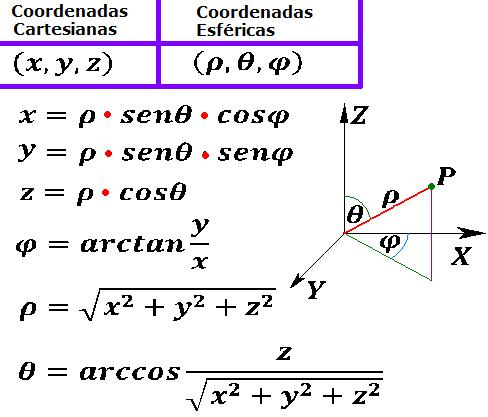
\includegraphics[scale=0.5]{ce.JPG}
		\centering
	\end{figure}
	
	\[u = \varphi cos \theta sin \phi \]
	\[ v = \varphi sin \theta sin \phi \]
	\[ w = \varphi cos \phi \]

	\section*{Hughes-Hallet}
	In Exercises $1-6$, check whether p is a joint density function. Assume $p(x, y) = 0$ outside the region R.
	
	\textbf{Ejercicio 6} $p(x, y) = xye^{-x-y}$, where R is $x \geq 0$, $y \geq 0$
	
	\s
	
	Para decir que p es una funci\'{o}n de densidad debe de cumplir 
	\begin{itemize}
		\item $p(x, y) \geq 0$
		\item $\iint_R p(x, y) \, \text dA = 1$
	\end{itemize}

	$\rightarrow$ Probemos que $p(x, y) \geq 0$:
	
	Se tiene que $x \geq 0$, $y \geq 0$ entonces $e^{-x-y}$ es positivo para cualquier punto $(x, y)$ en R
	
	Por lo tanto $p(x, y) \geq 0$
	
	$\rightarrow$ Probemos que $\iint_R p(x, y) \, \text dA = 1$:
	
	\[ \int_0^\infty\int_0^\infty xye^{-x-y} \, \text dx \, \text dy  
	  = \int_0^\infty y \left( -e^{-y-x}x-e^{-y-x}\right) \Big|_0^\infty dy\] 
	\[= \int_0^\infty y\left(\left( -e^{-y-\infty}\infty-e^{-y-\infty}\right)- 
		\left(-e^{-y-(0)}\cdot(0)-e^{-y-0}\right)\right)dy \]
	\[= \int_0^\infty y \left((0)\cdot \left( -e^{-y-(0)}\cdot(0)-e^{-y-0}\right)\right)dy\]
	\[= \int_0^\infty y \left(-\left( -e^{-y}\right)\right) dy\]
	\[= -e^{-y}y-e^{-y}\Big|_0^\infty\]
	\[= -e^{-\infty}\infty-e^{-\infty} -\left(-e^{-0}\cdot(0)-e^{-0} \right)  \]
	\[= 0 - \left(0-e^{0}\right)\]
	\[= 0 -\left(-e^{0}\right)\]
	\[= e^0 \]
	\[= 1\]
	
	Por lo tanto $\int_0^\infty\int_0^\infty xye^{-x-y} \, \text dx \, \text dy = 1$
	
	\textbf{Ejercicio 22}
	Two independent random numbers $x$ and $y$ between 0 and 1 have joint density function
	\[p(x,y) = \left\lbrace 
	 1 \, \,\text{if} \,\, 0 \leq x, y \leq 1 \atop 0 \qquad \text{otherwis}.
	\right. \]
	
	(a) Find $F(t)$, the probability that $z \leq t$. Treat separately
	the cases $t \leq 0$, $0 < t \leq 1/2$, $1/2 < t \leq 1$,
	$1 < t$. Note that $F(t)$ is the cumulative distribution
	function of z.
	
	\s 
	
	 Como $z \leq  t $ entonces cuando $t \leq 0$ $F(t) = 0$ pues $z=\frac{x+y}{2} \geq 0$ y cuando $t >1$ entonces $F(t)=1$ pues $z \leq 1$.
	\\
	Para el caso $0 \leq t \leq 1$ tenemos que $F(t)= \int_{R} p(x,y) dA$ donde $R$ es la región donde $\frac{x+y}{2} \leq t$, además como $p(x,y)=1$ solo si $0 \leq x, y\leq 1$ y$p(x,y)=0$ en otro caso, la integral solo tiene valor si $0 \leq x, y\leq 1$ .  Si hacemos que $t = \frac{x+y}{2}$ entonces tenemos que $F(t)$ es  el área dentro de la región que está debajo de la recta $t$. Se observa que $2t = x+y$ y cuando $x=0$ tenemos $y = 2t$ y cuando $y=0$ tenemos que $x = 2t$, por lo tanto $t$ junto con los ejes construyen un triángulo rectángulo de base y altura $2t$. 
	
	Cuando $0<t\leq \frac{1}{2}$ el triángulo está dentro de R pues $2t \leq 1$. Entonces $F(t) = \frac{2t*2t}{2}=2t^2$
	
	Cuando $\frac{1}{2} < t \leq 1$ no todo el triángulo está dentro de R pues $2t \leq 2$. Cuando $y=1$ tenemos que $x = 2t -1$ y cuando $x=1$, $y = 2t-1$, entonces la recta $t$ corta los límites de R en $x,y=2t-1$ lo que nos crea un triángulo rectángulo sobre $t$
	y dentro de R cuya base y altura es $1-(2t-1) = 2 - 2t$ y su área es $\frac{(2-2t)^2}{2}$. Por lo tanto $F(t) = 1*1 - \frac{(2-2t)^2}{2}=1-1-2t+t^2 =2t+t^2$
	\
	Por lo tanto, 
	\[
	F(t)=
	\begin{cases}
	0 & \text{si $t \leq 0$} \\
	2t^2 & \text{si $0<t\leq \frac{1}{2}$}\\
	2t+t^2 & \text{si $\frac{1}{2} < t \leq 1$}\\
	1 & \text{si $t>1$}
	\end{cases}
	\]
	
	(b) Find and graph the probability density function of z.
	
	\s 
	
	Obtenemos la función de densidad derivando la función acumulada. Entonces:
	\[
	f(t)=
	\begin{cases}
	0 & \text{si $t \leq 0$} \\
	4t & \text{si $0<t\leq \frac{1}{2}$}\\
	2+2t & \text{si $\frac{1}{2} < t \leq 1$}\\
	0 & \text{si $t>1$}
	\end{cases}
	\]
	
	
	(c) Are $x$ and $y$ more likely to be near $0$, $1/2$, or $1$?What about z?
	
	\s 
	
	Como $0 \leq x, y \leq 1$ es igual de probable que $x$ y $y$ estén cerca del 0, $\frac{1}{2}$ ó 1.
	
\end{document}